\documentclass[12pt]{article}

\usepackage{tgtermes}
\usepackage{epsf}
\usepackage{epstopdf}
\usepackage{amsmath}
\usepackage{graphicx}
\usepackage{booktabs}
\usepackage[colorlinks=true,linkcolor=blue,citecolor=blue]{hyperref}
\usepackage{dcolumn}
\usepackage{amsmath, amsthm, amssymb}
\usepackage{mwe}
\usepackage{url}
\usepackage{natbib}
%\usepackage{harvard}
\usepackage{fancyheadings}
\usepackage{longtable}
\usepackage{authblk}
\usepackage{setspace}
%\usepackage[nomarkers]{endfloat}
\usepackage{float}
\usepackage{bbm}
%\usepackage{titling}
\usepackage{subcaption}
\usepackage{algorithm}
\usepackage{algorithmic}
\usepackage{import}
\usepackage[backend=biber,style=authoryear,
sorting=ynt,citestyle=authoryear]{biblatex}
\addbibresource{papercitations.bib}
%\usepackage[nomarkers,nofiglist,notablist]{endfloat}

\onehalfspacing
\textwidth 6.5in \oddsidemargin 0in \evensidemargin -0.6in
\textheight 8.5in \topmargin -0.2in

\newcolumntype{L}[1]{>{\raggedright\let\newline\\
		\arraybackslash\hspace{0pt}}m{#1}}
\newcolumntype{C}[1]{>{\centering\let\newline\\
		\arraybackslash\hspace{0pt}}m{#1}}
\newcolumntype{R}[1]{>{\raggedleft\let\newline\\
		\arraybackslash\hspace{0pt}}m{#1}}
\newcolumntype{P}[1]{>{\raggedright\tabularxbackslash}p{#1}}

\newtheorem{theorem}{Theorem}[section]
\newtheorem{corollary}[theorem]{Corollary}
\newtheorem{proposition}[theorem]{Proposition}
\newtheorem{lemma}[theorem]{Lemma}

\captionsetup{justification=raggedright,singlelinecheck=false}


\newcommand{\xsub}[1]{%
	\mbox{\scriptsize\begin{tabular}{@{}c@{}}#1\end{tabular}}%
}

%\renewcommand{\thetable}{\Roman{table}}

\begin{document}
	
	
	
	
	\linespread{1.2}\title{\vspace{-0.5in} Does Hospital Leadership Matter?\\ \large Evidence from the Hospital Readmissions Reduction Program} 
	
	\date{\today}
	
	\author{\vspace{10mm}Hanna Glenn\footnote{Department of Economics, Emory University, 1602 Fishburne Drive, Atlanta, GA 30322, hanna.glenn@emory.edu.} }
	
	\maketitle
	%\setlength{\droptitle}{-10pt}
	
	\vspace{-0.2in}
	
	\singlespacing\maketitle

    \begin{center}
    \large
    \textbf{This is a preliminary draft. Please do not cite or circulate.}
	\end{center}

 \vspace{3mm}
	
    \begin{abstract}
		{\small
		The objectives that underlie nonprofit firm behaviors are not well understood, but perhaps that is because there are characteristics even within nonprofits that dictate behavior. In this paper, I use a novel data set on nonprofit hospital executives in the US from 2009-2015 to investigate whether having clinical experience on a hospital executive team affects hospital behavior. In particular, I leverage the Hospital Readmissions Reduction Program of 2012 as a shock to similar quality hospitals, and estimate the difference in response from hospitals with and without clinical experience. I find that while all penalized hospitals decreased readmissions after the shock, non-clinical executive team hospital decreased readmissions at a faster rate than those with a clinical executive team. The difference equates to approximately 15 additional readmissions for clinical team hospitals. I find no differential effect of clinical executive teams on mortality rates.
			
		} 
	\end{abstract}
	
	
	
	
	\vspace{0.8in}
	
	\noindent Keywords: 
	
	\noindent JEL Codes: 
	
	\onehalfspacing
	
	\newpage

  The objectives and behaviors of firms that are not classic for-profits are not easily determined, and an extensive literature has sought to understand these types of firms. Nonprofits are thought to gain utility not solely from monetary profit, but also through accomplishing mission-based purposes. Researchers have speculated a variety of objective functions that could motivate nonprofits such as maximizing prestige, income, or a quality/quantity tradeoff (Steinberg, 1986). An important contribution to this literature is the use of empirical strategies to analyze how firm behavior reveals attributes of the underlying objective function (\cite{sloan2000not}). In this paper, I leverage a large-scale shock to nonprofit hospitals in the US to investigate whether characteristics of the objective function are revealed by the composition of their leadership team.
  
  Hospitals in particular have been a common focus when seeking to understand not-for-profit firms. This is because, first, there are different hospital ownership types within the industry, giving researchers the ability to compare the behaviors of nonprofits with that of for-profits. Second, nonprofit hospitals make up 50\% of all hospitals in the US, and staff, on average, 207 beds. For comparison, for-profits make up around 36\% of hospitals and staff 107 beds (\cite{ASPE_2023}). Thus, nonprofit behavior in the hospital industry is relevant and directly affects consumers of health care. However, it remains unclear what type of objective function drives nonprofit hospitals (\cite{erus2002inferring}; \cite{deneffe2002not}; \cite{horwitz2009hospital}). 
  
  What has not been considered is how the leadership team within nonprofits potentially drives objectives. In large, publicly traded firms, executive characteristics are shown to be correlated with firm performance, indicating that there is more to firm behavior than just for-profit or not-for-profit status. Within nonprofit hospitals, there is variation in the propensity to hire executives with a background in clinical work, which could reasonably change how much weight the hospital places on profit vs. quality of care in their objective function. I contribute to our understanding of hospital and nonprofit behaviors by investigating whether clinical experience on an executive team affects hospital behavior after being financially penalized.

  Using publicly available tax forms, I construct a novel data set of nonprofit hospitals from 2009-2015 which captures the identities of executives tied to that hospital. I link hospitals in this data to characteristics in the American Hospital Association survey and Hospital Compare data. In order to capture the effect of clinical executives, not just their selection into certain types of hospitals, I specifically investigate hospitals penalized by the Hospital Readmissions Reduction Program (HRRP) of 2012. This program reduced Medicare payments to hospitals with above average readmission rates, and is plausibly uncorrelated with previously determined leadership teams. I further limit the sample to hospitals with stable executive teams over time, and characterize hospitals as having clinical experience on their team or not. 
  
  I estimate the difference in readmission and mortality rates between hospitals with and without clinical experience before and after the penalties began, conditional on being penalized. While readmissions directly affects the likelihood of being penalized, mortality rates are an explicit quality measure unrelated to the penalties. Including this as an outcome can help distinguish whether hospitals are improving quality or taking measures to only reduce readmissions. 
  
  I assume that before the penalty, clinical and non-clinical team hospitals behaved similarly along quality dimensions, and that the composition of hospital executive teams determined prior to the penalties is, conditional on being penalized, exogenous. Under these assumptions, I identify the effect of having a clinical executive on response to the penalty. I find that while both types of hospitals, those with clinical executives and those without clinical executives, decrease readmissions after being penalized, non-clinical team hospitals decrease readmissions at a faster rate. The difference equates to approximately 15 additional readmission cases per year for clinical teams, and there is no evidence that this result is driven by differences in readmissions prior to penalties. I find no differential effect of the program on mortality rates. 

    This paper contributes to three strands of literature. First, it adds to our understanding of what underlies nonprofit hospital behavior. This literature is extensive, and a review of it is beyond the scope of this paper. To summarize, there are various aspects of nonprofit behavior and objectives for which the evidence of how much it differs from for-profits remains mixed: costs, uncompensated care, technology adoption, and quality (\cite{sloan2000not}; \cite{eggleston2008hospital}; \cite{moscelli2018effect}; \cite{moscone2020public}). What underlies this is the need to understand the ways in which nonprofits make choices differently than for-profits. To this point, researchers have found that nonprofits do not act as purely profit maximizers, but maximize some combination of profit and output (\cite{deneffe2002not}, \cite{chang2011nonprofit}). A paper with a similar methodology to investigate hospital behavior is \citeauthor{chang2011nonprofit} (\citeyear{chang2011nonprofit}), which looks at the effect of a cost shock on likely of shutting down and mix of profitable services. They find that nonprofits and for-profits are equally as likely to shut down after the shock, but only nonprofits adjust their mix of profitable services. Similarly, I investigate a financial shock to hospitals, but I look at the differential impacts of leadership teams within nonprofits. This paper adds to our understanding of inputs into nonprofit hospital objective functions, and whether this is dependent on leadership compositions. 

    Second, many researchers have documented a correlation between executive backgrounds and firm performance specifically for CEOs, starting with \citeauthor{bertrand2003managing} (\citeyear{bertrand2003managing}), who show that manager fixed effects are an important driver of many firm behaviors and decisions. Female board members are associated with better oversight and more women executives (\cite{matsa2011chipping}; \cite{adams2009women}), but are negatively correlated with firm value (\cite{ahern2012changing}). Having more female executives is correlated with female employee wages and corporate strategies (\cite{flabbi2019female}; \cite{matsa2013female}); young male CEOs tend to be more aggressive in mergers and acquisitions while those with military experience are less aggressive (\cite{levi2010deal}; \cite{benmelech2015military}); CEOs with general ability tend to receive higher pay and perform better (\cite{kaplan2012ceo}; \cite{custodio2013generalists}, \cite{adams2018director}; \cite{frydman2019rising}). Further, Chief Diversity Officers are not found to have any effect on hiring more diversely in universities (\cite{bradley2022impact}). Due to data limitations, these studies focus mostly on large, publicly traded firms in the US. However, one study uses data from England to study whether CEOs affect hospital production, and find no association (\cite{janke2019impact}). I contribute to this literature first by investigating a context which is not largely studied but is policy relevant, nonprofit US hospitals, and considering a unique executive characteristic pertinent to that context. Second, I contribute by addressing leadership team endogeneity concerns through leveraging a shock to hospitals and strategically limiting the sample. 

    Finally, I contribute to our understanding of how providers respond to pay-for-performance incentives in health care. The most in depth study of how hospitals respond to HRRP is \citeauthor{gupta2021impacts} (\citeyear{gupta2021impacts}). The author finds that hospitals decreased readmissions by 5\% and mortality rates by 2\% on average as a result of the program, confirming prior studies (\cite{mellor2017does}; \cite{ziedan2018essays}; \cite{ody2019decreases}; \cite{gupta2021impacts}). Importantly, around 40\% of the decrease in readmissions is due to selective patient practices. This raises important questions about how to incentivize improvement in quality of care without also incentivizing gamesmanship. This paper addresses a necessary first step in considering whether leadership compositions could affect likelihood of gaming, which is to first investigate whether leadership matters to hospital decisions at all. 

    

    \section{Institutional Setting}

    \subsection{Hospital Readmissions Reduction Program}\label{sec:hrrp}

    The Hospital Readmissions Reduction Program (HRRP) was passed as a part of the Affordable Care Act in 2010 as a pay-for-performance incentive for hospitals to increase quality. In 2011, the Center for Medicare and Medicaid Services (CMS) released a set of rules that mandated penalties for hospitals with above average readmission rates. A readmission is when a patient returns to the hospital within 30 days of being discharged from a previous stay; avoidable readmissions are a bad outcome for patients and increase health care spending. The goal of HRRP is to lower readmissions through better care coordination, less initial stay complications, and better post-care instructions. Beginning in October 2012, hospitals with higher readmission rates than the national average in pneumonia, heart failure, or AMI (after adjusting for demographic characteristics) receive a lower reimbursement rate for Medicare patients. In 2015, CMS also included chronic obstructive pulmonary disease, coronary artery bypass graft surgery, and elective primary total hip arthroplasty and/or total knee arthroplasty as conditions which go into the penalty calculation. 
    
    Penalized hospitals pay a flat rate for every Medicare patient, not just those for which they have too high readmissions. Further, CMS does not distinguish a necessary readmission vs. an avoidable readmission, any repeat hospital visit is included in the penalty calculation. Excess readmission rates are calculated using a rolling look-back period of 3 years to determine whether the hospital is penalized. Therefore, hospitals had incentive to react immediately once details of the program were announced in October of 2011. These penalties are not insignificant; penalized hospitals paid, on average, 4-5\% of revenue. 

    \subsection{Nonprofit Hospital Leadership}

    Nonprofits are governed by a board of directors, whose role is to set high level goals and strategies, and provide general oversight. The board is not in charge of day-to-day operations, but the general direction of the firm. They select members of the executive team to carry out day-to-day operations. While hospital executives typically do specialize by getting degree(s) in healthcare management or an MBA specific to healthcare, they do not often have hands on clinical experience. When there is a hospital executive with clinical experience, they likely decided on that career path after becoming a doctor. While some doctors earn additional degrees before stepping into an executive role, this is not a necessary condition to becoming a physician executive. An executive team usually consists of at least a CEO and CFO. Every nonprofit is different in exactly how they structure an executive team. Some nonprofits hire Chief Medical Officers, Chief Quality Officers, executive directors, vice presidents of various departments, etc. I consider all of these employees as part of the day-to-day management of the hospital and include them as a part of the executive team. 

    All tax-exempt organizations in the US are required to file a Form 990 with the IRS each year. There are different types of forms, but any organization that grosses over \$200,000 must file the most extensive form 990. Sections of the form include a statement of revenue, statement of functional expenses, a balance sheet, and, as used in this project, a list of all key employees, executives, and board members. In this section, each firm is required to report the name and title, average hours per week, position, and compensation of their board members and executive leaders. Since these firms are tax exempt, their financial information is made publicly available through the public housing of these forms.  

  
	
	\section{Data}\label{sec:data}

    \subsection{Names of Hospital Leaders}

    To characterize hospitals as having clinical experience on their executive team or not, I construct a novel data set of nonprofit hospitals in the US that contains names and select characteristics of executives tied to the hospital from 2009-2015. I gather this data from each hospital's publicly available Tax Form 990, which every sufficiently large nonprofit files each year in the US. To my knowledge, this is the first large scale gathering of leadership names from these forms. 

    The historical tax forms for all nonprofits are housed by ProPublica\footnote{https://projects.propublica.org/nonprofits/}. I use the NonProfit Explorer API to extract the Employee Identification Numbers (EIN) of all nonprofits classified as a hospital according to their National Taxonomy of Exempt Entities (NTEE) code. After filtering out associations and specialty hospitals, there are around 3,000 firms left. Importantly, I need to be able to link hospitals in the tax forms to other hospital characteristics, including penalty status and readmission rates, in the American Hospital Association annual survey and Hospital Compare data. No official crosswalk between EINs and AHA IDs or Medicare numbers exists, so I must rely on matching by location and name of hospital in both data sets. After limiting to only general, nonprofit hospitals in the AHA survey, I confidently match approximately 1200 EINs to an AHA identification number based on exact name matches within the same state. 
    
    For each of the 1200 EINs, I extract web URLs to Form 990 PDFs in each year. I download these locally and use optical character recognition (OCR) text extraction methods to scrape the relevant section of the pdf, which is titled ``Officers, Directors, Trustees, Key Employees, and Highest Compensated Employees". Finally, I use string cleaning methods to identify names and positions for each EIN, year. I also identify titles indicating a physician: md, dr., or do. Using OCR extraction can be unreliable in some instances when the text is handwritten or the font is too small. Therefore, I manually find names, positions, and titles for observations that are missing after the initial extraction. This yields 850 EINs that are matched to AHA data, and are not missing text information. 

    Due to the lack of consistency in organization of executive teams, I focus mainly on the executive teams as a whole instead of specific positions. I drop anyone who is solely a board member, and focus on those who have executive in their title or are labeled as a president or vice president of a specific aspect of the hospital. My identification strategy relies on hospitals that have stable executive leadership over time. The ideal set of hospitals would be those who have the same executives on their team for the entire sample, as changes could be correlated with the fact that the hospital is penalized. However, this rarely occurs in reality. Therefore, I attempt to proxy for a stable leadership team while still having a large enough sample to run an analysis. Since my focus is clinical experience, my preferred specification is to limit the sample to hospitals who do not change the presence of a doctor on their leadership team from 2010-2014 (2 years before and after the program began). I make this limitation to hospitals in the sample and am left with 524 stable hospitals over time. Finally, I aggregate the information up to the hospital level, where an observation captures whether the hospital has clinical experience on their executive team over the course of the sample. 


    \subsection{Other Hospital Characteristics and Outcomes}

    I merge the leadership information with the AHA survey using the EIN-AHA links I created. From AHA, I gather the number of beds in the hospital and the Medicare number, which I use to merge the Hospital Compare data. Hospital Compare contains multiple data sets which I use first to limit to hospitals that were penalized in the Hospital Readmissions Reduction Program (HRRP), and also for information on my outcome variables, yearly readmission rates for the relevant HRRP conditions: heart failure, heart attack (AMI), and pneumonia.

    The Hospital Compare excess readmissions files contain information on the excess readmission measure used by CMS to determine whether a hospital should be penalized. Specifically, CMS calculates the average readmission rate of all hospitals, adjusts for demographic factors, and determines the amount of readmissions a hospital has in excess to of the average. This variable is condition specific, where a hospital is penalized if any of the three excess readmission ratios are greater than one\footnote{Additional conditions were added to the penalty calculations in 2015, but I do not consider these since my sample does not extend past 2015}. Further, Hospital Compare also publishes hospital level readmission and mortality rates for heart failure, AMI, and pneumonia. For my main outcomes of interest, I take an average across conditions and weight it using the total number of patients seen for that condition. For further analysis, I create samples of hospitals who were penalized for specific conditions, and investigate the change in readmission and mortality rates for the condition they were penalized in.

    \import{Tables}{noMDchg_sumstats.tex}

    In Table \ref{tab:sumstats}, I present summary statistics for various hospital characteristics including which condition hospitals are penalized for, and the readmission and mortality outcome variables. After limiting to penalized hospitals with stable leadership teams, my sample consists of between 302-310 hospitals from 2009-2015, except in the case of AMI outcomes, which is only 225-264 hospitals due to small patient numbers. Fourteen percent of hospitals have someone with clinical experience on their executive team, and the size of the hospitals in the sample varies quite a bit. The average number of beds for a hospital in the sample is 186, only slightly lower than the national average for all nonprofits. Hospitals in the sample are less likely to be penalized for AMI than either heart failure or pneumonia. On average, 21\% of patients with one of these conditions would be readmitted. While readmission rates for the specific conditions are similar, the highest likelihood of readmission is for heart failure patients. Alternatively, AMI is the most dangerous condition in terms of mortality rates. 

    Figure \ref{fig:weighted_read_mort_graph} shows average readmission rates for hospitals in the sample across time and across the three different conditions plus the weighted average. There are multiple notable points the raw data reveals. First, prior to the penalty, hospitals without clinical executives had consistently higher readmission rates than clinical executive hospitals across all conditions. While there is a gap between clinical team and non-clinical team readmission rates, the lines seem to move mostly parallel. In contrast, 2012 begins a decline in readmission rates over all conditions for all types of hospitals. This makes sense and is consistent with previous literature on HRRP, as hospitals have incentive to reduce readmissions in order to reduce future penalties. However, non-clinical hospital teams decrease readmissions at a faster rate, quickly converging with the rates of clinical team hospitals. While suggestive, this motivates further analysis into the differential responses between clinical and non-clinical leadership teams. 

    \begin{figure}[ht!]
        \caption{Readmission rates over time in all penalized hospitals}
        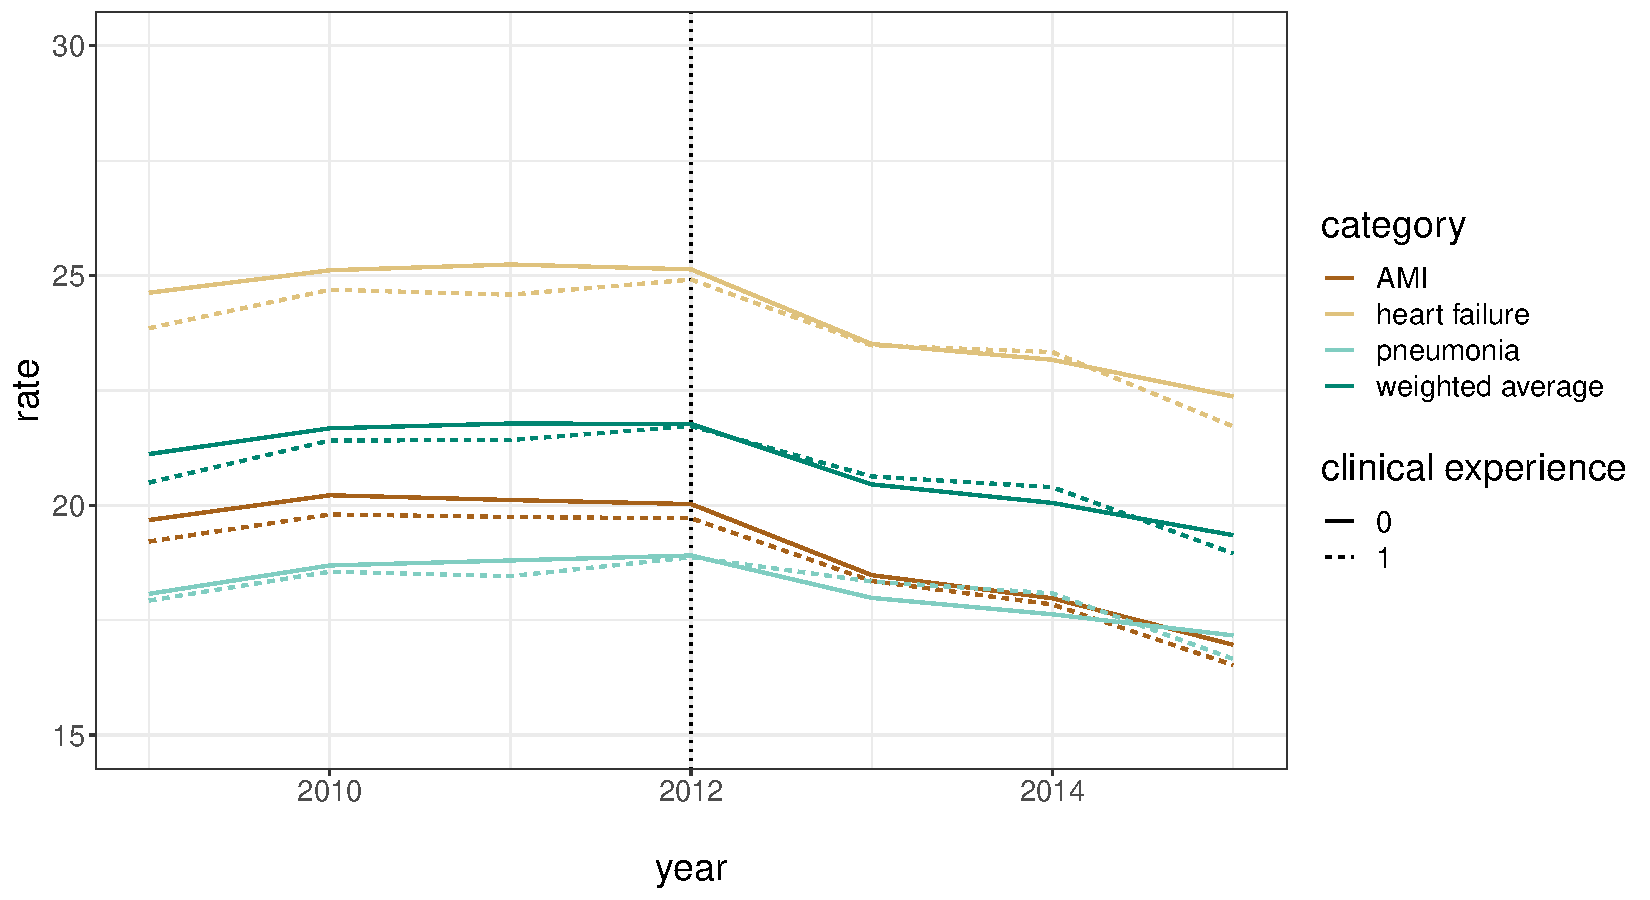
\includegraphics[scale=.55]{Objects/weighted_read_graph.pdf}
        \label{fig:weighted_read_mort_graph}
    \end{figure}

    \section{Model and Empirical Strategy}

    Not knowing the true form of nonprofit hospital objective functions, we can assume that they maximize some weighted average of revenue and output. Abstracting away from quantity for the purpose of this paper, we can think of firms behaving according to:     
    
    $$\max\hspace{2mm} \delta R + (1-\delta) u(\theta),$$

    \noindent where nonprofits differ from for-profits in that $\delta\neq 1$. Then $R$ is net revenue, $u(.)$ is an increasing function that captures utility from quality of care, and $\theta$ is some quality of care measure. In this setting, we care about hospital responding to a penalty by adjusting readmission rates, so $\theta = 1-r$, where $r$ is the readmission rate. While previous research has set out to understand the average $\delta$ for nonprofit hospitals, $\delta$ may also be dependent on the leadership teams within nonprofit hospitals. Further, introducing the HRRP means that $R$ is directly dependent on $\theta$. We can then write the hospital's problem as 

    $$\max\hspace{2mm} \delta(L) R(\theta) + (1-\delta(L)) u(\theta)$$

    \noindent where $L$ captures the composition of the leadership team. Therefore, when maximizing this function, the choice of $\theta$ is dependent on $L$ through its impact on how the hospital values profit vs. quality of care.

    Thus, I directly estimate the effect of having clinical experience on readmission rates. However, looking purely at this correlation is a biased picture of the effect of clinical experience since it likely captures reverse causality: certain types of hospitals may be more likely to hire doctors as executives. I do two things to address this issue. First, as discussed in detail in Section \ref{sec:data}, I only consider hospitals with stable leadership teams over time. Second, I leverage the HRRP shock, limiting the sample to those that were penalized, which allows me to identify hospitals similar in quality along readmission rates, and to observe changes in behavior after the shock. For the hospitals in my sample, I define their type as having clinical experience on their executive team or not, a time invariant categorization. 

    I estimate the following regression equation:

    \begin{equation}
    \label{eq:main}
    y_{ht} = \beta (clinical \times post\_penalty)_{ht} + \alpha_{h} + \delta_t + \epsilon_{ht}
    \end{equation}

    \noindent where $y_{ht}$ is one of the outcome variables discussed in Section \ref{sec:data}, $\beta$ is the variable of interest capturing the effect of having clinical experience after the penalties took place, $\alpha_h$ and $\delta_t$ are hospital and time fixed effects, respectively. As discussed in Section \ref{sec:hrrp}, hospitals had incentive to decrease readmissions immediately when the rules were released in October of 2011, before the penalties were actually determined in October of 2012. However, I still define $post\_penalty$ as occurring in 2012 or later, the first full year when hospitals would want to respond. 

    For identification, I rely on the assumption that, prior to being penalized, clinical and non-clinical team hospitals did not differentially change readmission rates for a reason I do not capture here. I investigate this assumption by estimating event study coefficients, where the coefficients $\beta_j$ now capture the effect of having clinical experience in a particular year, and $\beta_{2011}$ is normalized to zero:

    \begin{equation}
    \label{eq:es}
    y_{ht} = \sum_{j=2009}^{2010}\beta_j(clinical_{ht} \times \mathbf{1}\{y=j\}) + \sum_{j=2012}^{2015}\beta_j (clinical_{ht} \times \mathbf{1}\{y=j\}) + \alpha_{h} + \delta_t + \epsilon_{ht}.
    \end{equation}

    \section{Results}

    \subsection{Readmission Rates}

    I present the estimated coefficient of interest from Equation \ref{eq:main}, $\beta$, in Table \ref{tab:mainresults}. In column 1, the outcome is the weighted average of readmission rates. The estimated effect of having clinical experience on the hospital's reaction to the penalty is .47, indicating that hospitals with clinical experience on their executive team have a .47 point higher readmission rate than non-clinical team hospitals after being penalized. Comparing this to an average readmission rate of 21, this is a difference of approximately 2\%. When considering an average total number of patients of 760, this is a difference of 15 readmissions per year. Based on previous studies and on Figure \ref{fig:weighted_read_mort_graph}, both types of hospitals decrease readmission rates after the penalties begin, so a positive $\beta$ indicates that non-clinical team hospitals decrease readmissions at a faster rate than clinical team hospitals. 

    \import{Tables}{read_results_table.tex}
    
    In columns 2, 3, and 4, I limit the sample to hospitals penalized specifically for the condition that matches the outcome in the model. The coefficients are consistent and similar to that of the weighted average coefficient. Therefore, one of the conditions is not driving the entire weighted average. While similar in magnitude, the estimate for $\beta$ with the outcome of AMI readmission rate is statistically insignificant. Out of all the outcomes, AMI is the most likely to be missing data due to insufficient number of patients, which could explain this. 

    Finally, I plot estimated coefficients from Equation \ref{eq:es} in Figure \ref{fig:wa_eventstudy}. The result is consistent with clinical team hospitals having higher readmissions post-penalty. The magnitude of the effect in the years after the penalty began are still around .5, but range from .26 to .54 from 2012-2014. Further, there is no indication that having clinical experience on the executive team causes a reaction in readmissions prior to the penalty. 


    \begin{figure}[ht!]
        \caption{Event Study Estimates}
        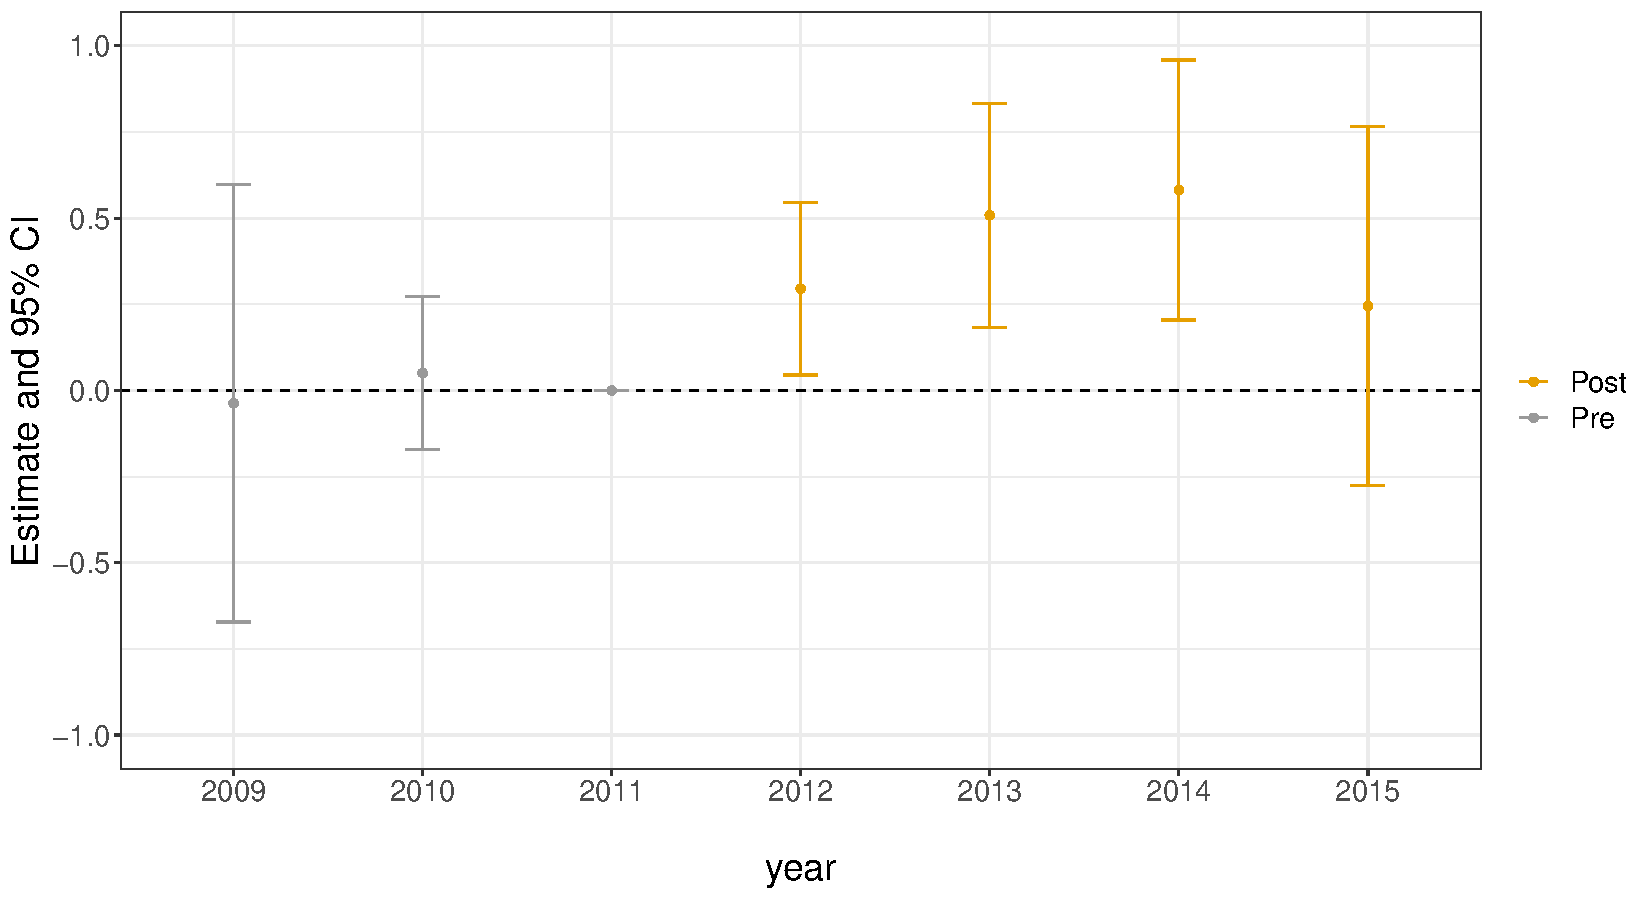
\includegraphics[scale=.5]{Objects/read_es_graph.pdf}
        \label{fig:wa_eventstudy}
    \end{figure}

    \subsection{Mortality Rates}

    \import{Tables}{mort_results_table.tex}

    \section{Conclusion}

    In this paper, I study the effect of having clinical experience within hospital leadership on nonprofit hospital behavior. Specifically, I leverage the Hospital Readmissions Reduction Program, which began in 2012, to identify similar quality hospitals along the dimension of readmission rates. For these similar hospitals, I estimate the difference in readmissions after being penalized between hospitals with clinical executives and hospitals without clinical executives. I find that while the penalty program led both types of hospitals to decrease readmissions after being penalized, those without clinical experience on their executive decreased rates more quickly than non-clinical team hospitals. 

    This finding reveals important information about hospital objectives, specifically that the composition of a hospital's leadership team affects the value placed on profit (or in this case, avoiding loss) vs. quality of care. Therefore, not-for-profit vs. for-profit status should not be the only characteristic considered by policymakers when designing incentives to increase quality of care. 

	
	\newpage

    \printbibliography

	% \appendix

 %    \section{Data}\label{appendixdata}

 %    \subsection{Gathering Hospital Leadership Names}

 %    There is no perfect way to access tax form 990s in bulk over the time period I am considering in this paper. However, using the NonProfit Explorer API seems to be the most straightforward. At the time of writing this, information on using version 2 of the API can be found at \hyperlink{https://projects.propublica.org/nonprofits/api}{https://projects.propublica.org/nonprofits/api}. 
    
 %    There are over 1.5 million nonprofit entities in the US (cite), making it crucially important to be able to filter by type of entity before analyzing any PDFs. The API allows this by filtering a query based on National Taxonomy of Exempt Entities (NTEE) code. I query only nonprofits categorized as E20 (hospitals), E21 (community health systems), and E22 (general hospitals). The API has a pagination limit of 100, meaning I can only pull information on 100 hospitals at a time. Therefore, I filter the query further to only consider one state at a time. The only state that has more than 100 entities registered is California, and thus I subset the California query even further by names that include the word "hospital" and names that don't. I combine all of these subsets and have information on each nonprofits Employee Identification Number. There are 5,588 EINs total in this list. This acts as a list of entities for which I can pull more information. 

 %    I loop through the list of EINs found in the previous step and query more detailed information from the API on that specific EIN. I save the name, secondary name, state, and zip code, all of which do not vary by year. I also save each year's URL that links to the Tax Form 990 PDF. For the sake of a comprehensive data set, I keep years 2006-2020 (I later limit to 2009-2016 when focusing on the Hospital Readmissions Reduction Program). Thus, I finish this step with a panel data set of EIN characteristics and PDF locations. Importantly, there are multiple types of Tax Form 990s depending on the size of the nonprofit. In many cases, one nonprofit has at least two different forms filed in a given year. I filter out any EIN-years for which there are no PDFs on file. The data on PDF locations contains 4,012 EINs and 61,363 EIN-year-tax forms.

 %    It is crucial to the analysis to be able to link these nonprofits with other sources of data to recover penalties from HRRP, bed size, and outcomes of interest (definitely need to talk more about outcomes). Therefore, I take a conservative approach to matching EINs to American Hospital Association (AHA) ID, which links fairly easily to Medicare ID numbers, based on name and location. First, I will discuss limitations and cleaning that I do to the AHA data and tax form data separately before doing any matching. 

 %    I download the AHA data from Wharton Research Data Services. I filter only to hospitals in the contiguous US, Alaska, and Hawaii (excluding places like Puerto Rico), classified as nonprofit or state/community, and those that are general acute care. I also filter out any hospitals who weren't present in the data (or change system ID) in 2009-2015, meaning they either closed or were acquired. Due to the survey nature of this data, a hospital name may look slightly different from one year to the next. For example, "Waldo County General Hospital" is also Waldo County General Hospital Maine Health". Further, zip codes may change by one or two digits, making them unreliable to match based on. To deal with this, I first keep only unique AHA ID, name, zip, state, and system name combinations. Then, I convert the data from long to wide so that each AHA ID occurs only once, but may have multiple names, zip codes, or system names associated with it.

 %    I consider which nonprofit entities are not likely to be hospitals and drop them. There are numerous foundations or auxiliary nonprofits with the purpose of raising funds for the hospital, but do not actually care for patient. I filter out any nonprofit with "foundation" or "auxiliary" in the name. I also filter out various specialty centers that fell into the general hospital category, such as hospice or cancer centers. 

 %    I then proceed matching based on names in multiple layers. I focus on exact string matches, so I remove all spaces and common characters that could cause mismatches such as \&, ', -, and inc. Next, I take each AHA name and look for exact matches in a nonprofit's first or secondary name only for nonprofits in the same state as the AHA hospital. When an exact match is found, I record the link between AHA ID and EIN. In this first layer of matching, 860 hospitals in the AHA data are linked to an EIN, equivalent to 31\% of AHA nonprofit hospitals in the sample. 

 %    In the next layer of matching, I remove common words such as "healthcare", "regional", "hospital", etc. That way if there are subtle differences in names, removing common words may allow for an exact match. Again, I take each AHA hospital name and look for exact matches in the nonprofits within the same state. This adds an additional 90 hospital matches, accounting for a total of 34.5\% of AHA hospitals. 

 %    In some cases, tax forms are associated with a system of hospitals instead of one individual hospital. Thus, I create another variable that captures the names of systems which match. The process of matching is the same, the only difference is that now I am considering system names from the AHA data instead of hospital names. A total of 1,136 AHA hospitals have an EIN match on hospital name, system name, or both. This is roughly 41\% of the sample. These hospitals become the main sample for my analysis. While not capturing a large majority of AHA hospitals that are categorized as nonprofit, I would rather be conservative in selecting hospitals which I am confident that the characteristics and measurement of the independent and dependent variables are accurate. 

 %    (add a paragraph about validity of matches)

 %    Now that I have a sample of hospitals, the next step is to extract the names of the people in charge of these hospitals from the Tax Form 990 PDFs. In the data set of hospital PDF URLs that I collected earlier, I limit to the hospitals with solid matches described above. I then loop through each EIN, downloading each PDF locally and using tesseract package in R to extract text from the relevant pages of the PDF using OCR text extraction methods. In particular, I loop through each page of the PDF, look for the title associated with leadership names: ``Officers, Directors, Trustees, Key Employees, and Highest Compensated Employees", and save all the text from any pages where this title is found. I save the text to a list of all EIN, years present. 

 %    One tricky aspect of the NonProfit Explorer API is that, only in some cases, if two forms are present for an EIN, year, only the first one (which is typically not the one with the relevant information) is pulled. Therefore, for some hospitals, a couple years will have gaps in text extraction data. I locate EIN, years where this problem is occurring, and a team of RAs locates and downloads the correct forms manually. I extract text from these manually downloaded forms in the same manner as above. 

 %    The form of the text data is a data frame with one column, where each line of text is saved in a different row. I write a text cleaning package that locates names, positions, titles, and indications of resigning. I will now describe this function in three parts: preliminary cleaning of strings, locating names, and locating positions, titles, and key words surrounding resigning. 

 %    Typically on the same page as the names and positions is a list of the highest compensated employees and their compensation. In order to not record extra names, I filter out any rows after the start of this section. I then remove any digits, parentheses and brackets, other punctuation, letters that occur by themselves, two letter ``words" that have no meaning, and excess space between words. I then split up the phrase into individual words, so one phrase with 5 words is broken up into 5 variables. 

 %    Next, I locate first and last names in the data. 


    

    

    

    

    

    

	
	
	


\end{document}

